\documentclass[11pt]{article}
% CS690A report format: LaTeX, single column, 11pt, 1-inch margins, at most 9 pages including references,
% appendix and the contribution statement (last page).
% Overleaf: upload main.tex, refs.bib and figures/; compile with pdfLaTeX + BibTeX.
% Figures: python paper/make_figures.py <ccc-nulls checkout>
\usepackage[margin=1in]{geometry}
\usepackage[utf8]{inputenc}
\usepackage[T1]{fontenc}
\usepackage{lmodern}
\usepackage{amsmath,amssymb}
\usepackage{graphicx}
\usepackage{booktabs}
\usepackage{tabularx}
\usepackage{caption}
\usepackage{float}
\usepackage[numbers,sort&compress]{natbib}
\usepackage{url}
\usepackage[hidelinks]{hyperref}
\graphicspath{{figures/}}
\captionsetup{font=small,labelfont=bf}
\setlength{\parskip}{3pt}
\newcommand{\JLP}{JLP}
\newcommand{\BPT}{BPT}
\newcommand{\MDT}{MDT}
\newcommand{\LOO}{LOO-$t$}
\newcommand{\st}{$s\!\to\!t$}

\title{\vspace{-1.2em}Bilateral Permutation Tests for Cell--Cell Communication}
\author{Kaushal, Kshitij Bhardwaj, Ankit, Aritra\\[2pt]
\small CS690A Computational Genomics, Project 6 \quad (mentor: Hamim Zafar)\\
\small Indian Institute of Technology Kanpur}
\date{November 2026}

\emergencystretch=1.5em
\begin{document}
\maketitle

\begin{abstract}
\noindent
Cell--cell communication (CCC) tools such as CellPhoneDB and CellChat attach a permutation p-value to every
sender~$s$, receiver~$t$ and ligand--receptor pair $(L,R)$, and that p-value is read as evidence that ``$s$ signals to
$t$ through $(L,R)$''. We show that their test, a joint permutation of all cell labels (\JLP), answers a weaker
question: it rejects when \emph{either} side is cell-type specific. On known nulls, where one side carries no signal,
\JLP's false discovery rate (FDR) is 27--100\% for all four tools we studied (CellChat, CellPhoneDB, Connectome,
NATMI). We propose a bilateral permutation test (\BPT) that permutes each side separately and rejects only if both
reject, and we compare it with two permutation-free alternatives through the same pre-registered tests. \BPT{} has an
FDR of at most 3.1\%. Inside LIANA+'s consensus ranking it lowers the false share of the top~1\% from 83--88\% to
61--78\% when it replaces CellChat's and CellPhoneDB's p-values, and to 42--47\% when it also replaces Connectome's
and NATMI's, while ranking planted interactions higher (AUROC 0.915 $\to$ 0.992). Both gains hold on a held-out
tissue and in mouse. Permuting within donor removes donor-driven false calls. No test is distinguishable on the
available spatial truths.
\end{abstract}

% =====================================================================
\section{Introduction and motivation}

Single-cell atlases are now routinely mined for cell--cell communication: which cell type sends a ligand that
another cell type receives. CellPhoneDB~\cite{efremova2020} and CellChat~\cite{jin2021} score every ordered pair of
cell types $(s,t)$ and ligand--receptor pair $(L,R)$ and attach a p-value obtained by shuffling cell labels.
LIANA+~\cite{dimitrov2022,dimitrov2024} runs several such methods and merges their rankings into one consensus.
The p-values decide which interactions are reported, and readers interpret a small one as ``$s$ talks to $t$ via
$(L,R)$''.

That interpretation requires two things at once: $L$ must be specific to $s$ \emph{and} $R$ must be specific to $t$.
The tools' test permutes all labels together, so its null is ``labels do not matter for either partner''. A ligand
that is specific to $s$ paired with a receptor expressed everywhere rejects that null for \emph{every} receiver $t$.
The test is exact; it simply tests a different claim. Simulations in which all data are permuted cannot separate the two readings, so we
test them on real data, with four tools and four competing tests.

We ask two questions, each with its own pre-registered benchmark:
\begin{enumerate}\setlength{\itemsep}{0pt}
  \item Are each tool's own p-values valid for the claim \st{} via $(L,R)$? (Benchmark~1, tool level)
  \item Does a valid test improve the ranking that users actually read, LIANA+'s consensus? (Benchmark~2)
\end{enumerate}
Our contributions are: an exact Python reimplementation of CellChat's and CellPhoneDB's test that matches the native
tools on every one of 10.4~million p-values; the bilateral permutation test (\BPT) and two permutation-free
alternatives, all available as one package; and a benchmark on five data sets, a held-out tissue and mouse, run from
a single commit with the decision rule fixed before any result was seen.

% =====================================================================
\section{Related work}

\textbf{CCC inference.} CellPhoneDB~\cite{efremova2020} and CellChat~\cite{jin2021} derive p-values from label
permutations; Connectome~\cite{raredon2022} and NATMI~\cite{hou2020} instead rank by a specificity score (a z-score of
ligand $\times$ receptor expression, and each side's share of its gene's expression across cell types) and report no
p-value. LIANA and LIANA+~\cite{dimitrov2022,dimitrov2024} re-implement these methods on a shared resource and
aggregate their ranks with robust rank aggregation~\cite{kolde2012}; LIANA's benchmark, now part of Open
Problems~\cite{openproblems}, found that methods disagree widely but did not ask whether any p-value tests the
two-sided claim. \textbf{Testing.} Permutation p-values should be computed as $(1+\#)/(B+1)$~\cite{phipson2010}. A
claim that needs two conditions is an intersection--union problem: the maximum of the two p-values is a valid test
with no multiplicity penalty~\cite{berger1982}. Gene-set tests against matched genes must correct for inter-gene
correlation, as CAMERA does~\cite{wu2012}.

% =====================================================================
\section{Methods}

\subsection{Four tests of the same score}
Let $S$ be a tool's score for one row $(s,t,L,R)$. All four tests take the tool's score as given and differ only in
the null they compare it with (Table~\ref{tab:names}).

\begin{itemize}\setlength{\itemsep}{1pt}
\item \textbf{Joint label permutation (\JLP)} is the tools' own test: shuffle all cell labels $B$ times, recompute
$S^*$, and report $p=(1+\#\{S^*\ge S\})/(B+1)$.
\item \textbf{Bilateral permutation test (\BPT)} shuffles only the sender side's labels to get $p_L$, then only the
receiver side's to get $p_R$, and reports $p=\max(p_L,p_R)$. It rejects only when both sides are specific, which is
the claim users make, and as an intersection--union test it needs no multiplicity correction.
\item \textbf{Matched-decoy test (\MDT)} ranks each side's gene against genes of matched mean expression and applies
CAMERA's correlation correction; no permutations.
\item \textbf{Leave-one-out $t$-test (\LOO)} compares a row's score with the same interaction's scores in all other
$(s,t)$ pairs; no permutations.
\end{itemize}
Calls are made by Benjamini--Hochberg at 5\%~\cite{bh1995}. All tests run on the tool's own score. For CellChat and
CellPhoneDB we compare with the native tools (CellChat 2.1.2 in R, CellPhoneDB 5.0.1); Connectome and NATMI have no
native p-value, so we run them inside LIANA+.

\begin{table}[H]
\centering\small\setlength{\tabcolsep}{3pt}
\caption{The four tests. The code uses the names in brackets.}
\label{tab:names}
\begin{tabular}{@{}lll@{}}
\toprule
Test & Rejects when & Permutations\\
\midrule
Joint label permutation, \JLP{} [Null A] & either side is specific & all labels (the tools' own test)\\
Bilateral permutation test, \BPT{} [Null B] & both sides are specific & each side separately (proposed)\\
Matched-decoy test, \MDT{} [Null B2] & both sides beat matched decoys & none\\
Leave-one-out $t$-test, \LOO{} [T2] & the pair beats the other pairs & none\\
\bottomrule
\end{tabular}
\end{table}

\subsection{Data}
Human: Tabula Sapiens~\cite{tabula2022} Mammary and Liver, and the TNBC atlas~\cite{wu2021} (10 patients). Mouse:
the Allen brain data set from Open Problems~\cite{openproblems} and the hypothalamus of Moffitt et
al.~\cite{moffitt2018}. Tabula Sapiens Lung (65{,}847 cells) was held out until the end. Biological truths are spatial
co-localisation (TNBC Visium, Allen brain, hypothalamus MERFISH) and downstream response
(CytoSig~\cite{jiang2021}, PROGENy~\cite{schubert2018}); the nulls always run on the single-cell data, and spatial data
are used only to score calls.

\subsection{Two benchmarks}
\textbf{Ground truth by construction.} We create \emph{known nulls} by shuffling one side's genes (all receptors, or
all ligands) across cells: every row then lacks a specific partner on that side, so every call is false. We create
\emph{planted pairs} by multiplying the expression of 30 ligand--receptor pairs by a fold change $f$ in one sender and
one receiver only.

\textbf{Benchmark 1 (tool level)} asks whether each tool's p-values are valid: FDR on known nulls, power and FDR on
planted pairs ($f=1.5$), calls on real data, and whether the calls a test keeps are more co-localised than those it
drops.

\textbf{Benchmark 2 (consensus)} asks whether the ranking improves. The baseline is LIANA+~1.8.0's five methods plus
CellChat with their own p-values (\JLP). Each test then replaces the p-values of CellChat and CellPhoneDB, then also
Connectome's and NATMI's specificities (the test is applied to their scores with the same permutations). We score the
share of the consensus' top~1\% that is false on known nulls, and the power and AUROC of planted pairs against rows
that are specific on one side only. The decision rule, fixed in advance, accepts a test if it is better calibrated
than the baseline, no worse in power, and both again on held-out Lung.

\textbf{Pre-registration and runs.} Two plans and thirteen amendments were each hashed (SHA-256) before their runs, and
every result file records the hashes. Benchmark~2 ran on Kaggle (143 sessions) and a lab server from one commit and a
locked environment, with $B=1{,}000$ permutations unless stated.

% =====================================================================
\section{Results}

\subsection{The tools' p-values are exact, but for the wrong claim}

We first had to rule out that any failure was ours. Our Python \JLP{} reproduces the native p-value on every row of
all five data sets and the native number of calls exactly (Table~\ref{tab:three}), so its behaviour is the tools'
behaviour.

\begin{table}[H]
\centering\small
\caption{Native tool, our Python reimplementation (\JLP) and \BPT, summed over five data sets.}
\label{tab:three}
\begin{tabular}{@{}llccc@{}}
\toprule
Tool & Measure & Native & Our Python (\JLP) & \BPT\\
\midrule
CellChat & p-values equal to native & -- & 4{,}623{,}511 / 4{,}623{,}511 & --\\
 & calls, tool's own rule & 64{,}173 & 64{,}173 & --\\
 & calls, BH 5\% & -- & 61{,}820 & 34{,}237\\
 & FDR on known nulls & -- & 0.27--0.75 & 0.00--0.03\\
\midrule
CellPhoneDB & p-values equal to native & -- & 5{,}824{,}308 / 5{,}824{,}308 & --\\
 & calls, tool's own rule & 130{,}499 & 130{,}499 & --\\
 & calls, BH 5\% & -- & 86{,}267 & 36{,}092\\
 & FDR on known nulls & -- & 0.96--1.00 & 0.00\\
\bottomrule
\end{tabular}
\end{table}

When one side's genes are shuffled, every call is false, yet \JLP{} still calls them: its FDR is 27--75\% for
CellChat and 91--100\% for CellPhoneDB, Connectome and NATMI (Fig.~\ref{fig:b1}a). \BPT{} keeps the FDR at or below
3.1\% for all four tools and \MDT{} at 0. \LOO{} fails as badly as \JLP{} (20--99\%), and it is the only test that
makes calls when \emph{all} labels are shuffled, on every tool. On real data \BPT{} keeps about half of \JLP's calls
(34{,}237 of 61{,}820 for CellChat, 36{,}092 of 86{,}267 for CellPhoneDB): the other half had only one specific side.

\begin{figure}[H]
\centering
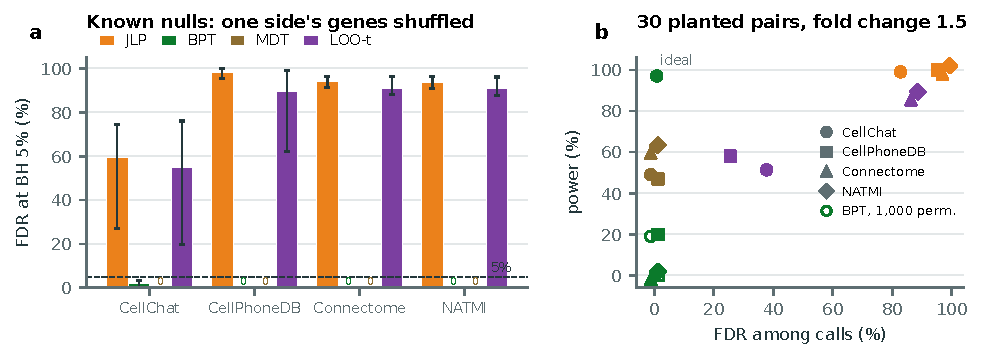
\includegraphics[width=\textwidth]{fig1_tool_level.pdf}
\caption{\textbf{Benchmark 1: each tool's own p-values.} (a) FDR at BH 5\% on known nulls (one side's genes
shuffled, so every call is false); bars are the mean over two tissues (Tabula Sapiens Mammary, Liver) and both sides,
whiskers the range; dashed line, 5\%. (b) Power against FDR for 30 planted pairs (fold change 1.5, BH 5\%, 5
replicates); colour is the test as in (a), shape the tool; \BPT{} filled, 5{,}000 permutations; open, 1{,}000.
Connectome and NATMI run inside LIANA+ and have identical values here; points are offset slightly to stay visible.}
\label{fig:b1}
\end{figure}

\subsection{BPT is valid, at the cost of more permutations}

Planted pairs show the price of each test (Fig.~\ref{fig:b1}b). \JLP{} finds every planted pair, but 84--98\% of
its calls are false. \BPT{} is the only test that reaches the ideal corner: with 5{,}000 permutations it finds 97\% of
CellChat's planted pairs at 2\% FDR. Its weak spot is resolution. Its smallest p-value is $1/(B+1)$, and across
millions of rows Benjamini--Hochberg needs smaller ones, so power is 0--19\% with $B=1{,}000$, 20\% for CellPhoneDB
even with 5{,}000, and zero in our LIANA+ runs (Connectome and NATMI, and CellChat and CellPhoneDB in the same runs).
\MDT{} finds about half of the pairs (47--61\%) without a false call; \LOO{} finds 51--87\%, at 24--87\% FDR. The tool-level picture is
therefore: \JLP{} and \LOO{} are not valid for the two-sided claim; \BPT{} and \MDT{} are, and \BPT{} has power if it
gets enough permutations.

\subsection{A valid test cleans LIANA+'s consensus, and more so the more tools use it}

Most users do not read one tool's p-values but LIANA+'s consensus, so the question that matters is whether a valid test
changes that ranking. Fig.~\ref{fig:b2} follows the false share of the top~1\% as each test replaces the p-values of
more tools. As shipped, 83--88\% of the top~1\% is false on known nulls. Giving CellChat and CellPhoneDB \BPT's
p-values lowers it to 61--78\% in all four data sets; giving Connectome and NATMI \BPT{} as well lowers it to
42--47\%, roughly halving the false share of the shipped consensus. The gain appears on held-out Lung (86\% $\to$
45\%) and in mouse (88\% $\to$ 44\%). \MDT{} helps less and, in human tissue, barely changes when Connectome and NATMI are added;
\LOO{} makes the ranking worse at every step.

\begin{figure}[H]
\centering
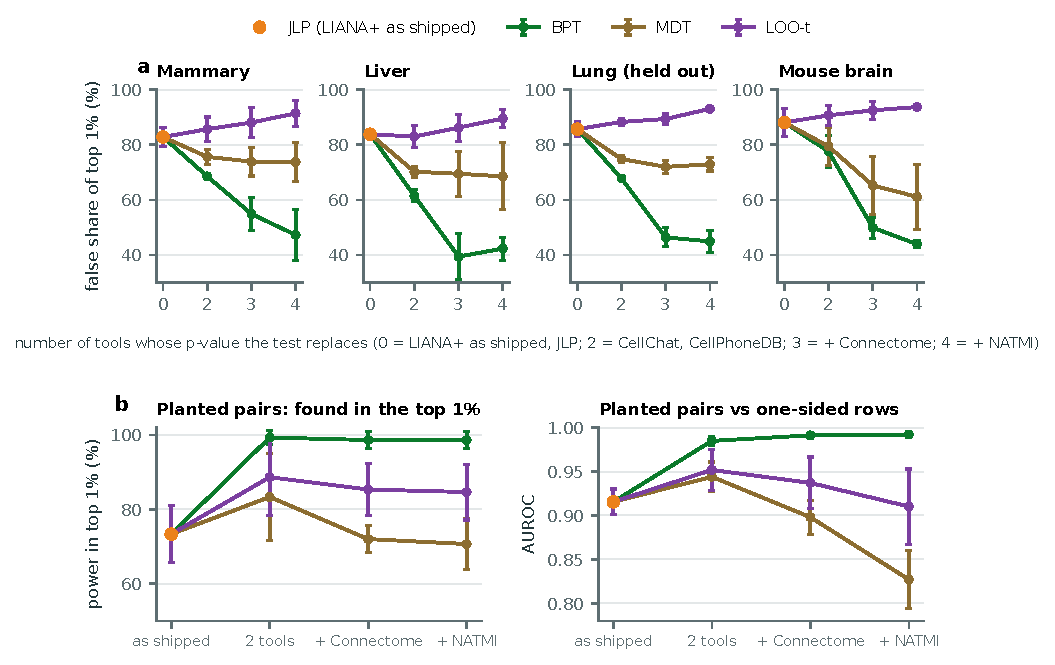
\includegraphics[width=\textwidth]{fig2_consensus.pdf}
\caption{\textbf{Benchmark 2: LIANA+'s consensus.} The x axis counts the tools whose p-value the test replaces:
0 = LIANA+ as shipped (\JLP, orange); 2 = CellChat and CellPhoneDB; 3 = also Connectome; 4 = also NATMI. (a) Share
of the consensus' top~1\% that is false on known nulls (receptors or ligands shuffled; mean and 95\% CI over 3
replicates of each). Lung was held out until the end; mouse is the Allen brain data set. (b) 30 planted pairs at
fold change 1.25 in Tabula Sapiens Mammary (5 replicates): share found in the top~1\% and AUROC against rows specific
on one side only.}
\label{fig:b2}
\end{figure}

The cleaner top does not cost power (Fig.~\ref{fig:b2}b). With \BPT, 99\% of planted pairs reach the top~1\% against
73\% as shipped, and the AUROC rises from 0.915 to 0.985 with two tools and to 0.992 with four. The mechanism is the
same as at tool level: rows with only one specific side no longer crowd the top, which leaves room for the pairs that
are specific on both sides. \MDT{} and \LOO{} lose power as more tools use them (AUROC 0.827 and 0.910 with four).
Under the pre-registered rule, \BPT{} is confirmed on held-out Lung with two, three and four tools' p-values replaced;
\MDT{} fails the power criterion once Connectome is included, and \LOO{} fails calibration every time.

\subsection{Donors, settings and biology}

\begin{figure}[H]
\centering
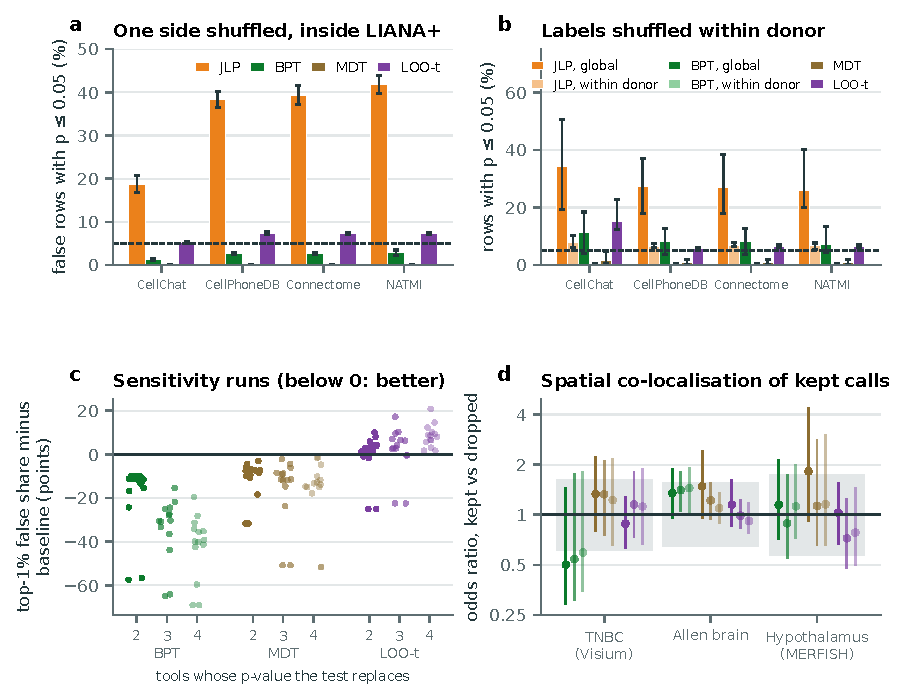
\includegraphics[width=0.9\textwidth]{fig3_robustness.pdf}
\caption{\textbf{Validity and robustness inside LIANA+.} (a) False rows with $p\le0.05$ when one side is shuffled
(Mammary and Liver, 12 runs; mean, 95\% CI); dashed line, the nominal 5\%. (b) Labels shuffled within donor, so there
is no cell-type signal: rows with $p\le0.05$, mean over four data sets (Lung, TNBC, Mammary, Liver), whiskers the
range; light bars permute within donor. (c) Each point is one sensitivity run (detection threshold, cell subsampling,
label resolution, 5{,}000 permutations, mouse): the test's top-1\% false share minus the baseline's; darker points
replace two tools' p-values, lighter three and four. (d) Among the baseline's calls, odds ratio of spatial
co-localisation for the calls a test keeps against those it drops (95\% CI); grey, the range not detectable with 80\%
power; within each test, shades as in (c).}
\label{fig:b3}
\end{figure}

Inside LIANA+ the p-values behave as at tool level (Fig.~\ref{fig:b3}a): with one side shuffled, 19--42\% of false
rows have \JLP{} $p\le0.05$, against 1.3--2.9\% for \BPT{} and 0.1\% for \MDT; \LOO{} sits just above nominal
(5.2--7.3\%). A second, unexpected source of false calls is donors (Fig.~\ref{fig:b3}b). When labels are shuffled
within donor, so that no cell-type signal remains, global permutations still give 18--51\% of rows \JLP{} $p\le0.05$
and 3.7--18\% for \BPT, because donor effects masquerade as cell-type effects. Permuting within donor brings \JLP{} to
5--10\% and \BPT{} to at most 0.6\%; our package now does this by default.

The improvement is not tied to one setting (Fig.~\ref{fig:b3}c): \BPT{} and \MDT{} beat the baseline in every one of
the 20 sensitivity runs with two tools and the 14 with three and four, \LOO{} in only 4, 4 and 0. \BPT's ranking is
as stable across seeds as the baseline's (top-1\% Jaccard 0.96--0.98).

Biology is where the evidence runs out (Fig.~\ref{fig:b3}d). Among the baseline's calls, the ones \BPT{} keeps are no
more co-localised than the ones it drops, and no spatial test is significant after BH for any test or number of
tools. With the available truths only odds ratios beyond 1.6--3 would have been detectable. The rows \BPT{} drops have a
broadly expressed limiting gene in all ten data set $\times$ tool pairs, which is exactly the one-sided pattern the test
is designed to remove.

\begin{table}[H]
\centering\footnotesize\setlength{\tabcolsep}{4pt}
\caption{Summary: every test through the same tests (\JLP{} = LIANA+ as shipped in Benchmark 2).}
\label{tab:summary}
\begin{tabularx}{\textwidth}{@{}Xcccc@{}}
\toprule
 & \JLP & \BPT & \MDT & \LOO\\
\midrule
FDR on known nulls, tool level (four tools) & 0.27--1.00 & $\le$0.03 & 0.00 & 0.20--0.99\\
Calls with all labels shuffled & none & none & none & always\\
Power / FDR, planted pairs, CellChat & 0.99 / 0.84 & 0.97 / 0.02 & 0.49 / 0.00 & 0.51 / 0.39\\
Top 1\% false, held-out Lung, 2 / 4 tools replaced & 0.86 & 0.68 / 0.45 & 0.75 / 0.73 & 0.88 / 0.93\\
AUROC of planted pairs, 2 / 4 tools replaced & 0.915 & 0.985 / 0.992 & 0.944 / 0.827 & 0.952 / 0.910\\
Rows $p\le0.05$, donor shuffles (global; within) & 18--51\%; 5--10\% & 3.7--18\%; $\le$0.6\% & 0.3--4.6\% & 5.5--23\%\\
Sensitivity runs beating the baseline & -- & 48 / 48 & 48 / 48 & 8 / 48\\
Pre-registered rule on held-out Lung & -- & confirmed & fails power & fails calibration\\
\midrule
Verdict & wrong claim & valid, confirmed & valid, few calls & not valid\\
\bottomrule
\end{tabularx}
\end{table}

% =====================================================================
\section{Discussion and limitations}

The tools' p-values are not wrong; they answer ``is at least one side specific?'', and the field reads them as ``are
both?''. Testing each side separately and taking the larger p-value answers the question users ask, keeps the FDR
below 5\%, and, because one-sided rows stop crowding the top, makes LIANA+'s consensus both cleaner and more
sensitive, more so the more of its methods use it (Table~\ref{tab:summary}). We therefore recommend \BPT{} with
within-donor permutations for any claim \st{} via $(L,R)$, with $B\ge5{,}000$ when Benjamini--Hochberg is applied.

\textbf{Limitations.} (i) Our biological truths are coarse: spatial proximity sees the pair, rarely the sender's
specificity, so we can show that \BPT{} removes false rows but not that the rows it keeps are more biological.
(ii) Two of LIANA+'s six methods (log2FC and SingleCellSignalR) still use no null. (iii) A filter requiring
differential expression on both sides removes even more false rows than \BPT, although \BPT{} ranks planted pairs
higher. (iv) \BPT{} needs about five times more permutations than \JLP{} to have power under BH.

% =====================================================================
\section{Data availability}

Tabula Sapiens (Mammary, Liver, Lung) is public on CELLxGENE~\cite{tabula2022}, and the hypothalamus single-cell
(GEO GSE113576) and MERFISH data come from Moffitt et al.~\cite{moffitt2018}. The TNBC atlas~\cite{wu2021} and the
Allen brain data set came from the Open Problems bucket~\cite{openproblems}, which closed in November 2026; our
copies, taken before it closed, are available from the team on request. The \texttt{code/} folder of the submission
holds the download scripts, the code, both plans, all thirteen amendments and every result file (each records the
commit, the plan hashes and the session or machine that produced it); its \texttt{README.md} gives the command for
every figure.

\bibliographystyle{unsrtnat}
{\footnotesize\setlength{\bibsep}{1.5pt}\bibliography{refs}}

% =====================================================================
\clearpage
\section*{Individual contribution statement}

All four members agree to this statement. Every member can answer questions on any part of the project.

\vspace{6pt}
\begin{center}
\renewcommand{\arraystretch}{1.35}
\begin{tabularx}{\textwidth}{@{}l l X@{}}
\toprule
Member & Roll No. & Contribution\\
\midrule
Kaushal & [roll no.] & Problem statement and data set selection; Connectome adapter for the tool-level benchmark.\\
Kshitij Bhardwaj & [roll no.] & Literature review (LIANA, LIANA+); CellChat reimplementation matched to the native test; the
bilateral permutation test; LIANA+ consensus pipeline and Benchmark 2 (plans, amendments, Kaggle and server runs);
report and slides.\\
Ankit & [roll no.] & Literature review (Open Problems, CellChat, CellPhoneDB); CellPhoneDB adapter with the native test;
named simulations; the leave-one-out $t$-test.\\
Aritra & [roll no.] & Literature review (NicheNet, Cauchy combination); NATMI through every stage of Benchmark 1; native
NATMI runs.\\
\bottomrule
\end{tabularx}
\end{center}

\vspace{18pt}
\noindent Signatures:\\[18pt]
\noindent\rule{0.2\textwidth}{0.4pt}\hfill\rule{0.2\textwidth}{0.4pt}\hfill\rule{0.2\textwidth}{0.4pt}\hfill\rule{0.2\textwidth}{0.4pt}\\
\noindent\makebox[0.2\textwidth][c]{Kaushal}\hfill\makebox[0.2\textwidth][c]{Kshitij Bhardwaj}\hfill
\makebox[0.2\textwidth][c]{Ankit}\hfill\makebox[0.2\textwidth][c]{Aritra}

\end{document}
